\documentclass[a4paper]{article}
\usepackage[margin=1in]{geometry}
\usepackage[T1]{fontenc}
\usepackage[utf8]{inputenc}
\usepackage[hidelinks]{hyperref}
\usepackage{amsmath, amssymb, amsthm}
\usepackage{graphicx}
\usepackage{listings}
\usepackage{xcolor}
\usepackage{booktabs}
\usepackage{caption}
\usepackage{ocgx2}
\usepackage{tcolorbox}


% Configuration pour les listings de code
\definecolor{codebg}{RGB}{245,245,245}

\lstset{
    backgroundcolor=\color{codebg},
    basicstyle=\ttfamily\footnotesize,
    frame=single,
    breaklines=true,
    columns=fullflexible,
    keywordstyle=\color{blue},
    commentstyle=\color{gray},
    stringstyle=\color{orange},
    showstringspaces=false,
    keepspaces=true,
    tabsize=4
}

%----- TITLE PAGE INFO -----%
\title{\Huge \textbf{Spanning Tree Protocol (STP) Workbook}\\
       \Large Fundamentals, Variants, Tuning, and Practical Labs}
\author{\Large Written for Networking Students and Professionals}
\date{\today}

\begin{document}

%----- MODERN TITLE PAGE -----%
\begin{titlepage}

	\centering
	\vspace*{4cm}
	{\Huge \textbf{EtherChannel}\par}
	\vspace{0.8cm}
	{\Large A Hands-On Guide to PAgP, LACP, and Static Aggregation\par}
	\vspace{0.3cm}
	\rule{0.9\textwidth}{1pt}

	\vspace{0.6cm}
	{\large \textbf{Mehdi JAFARI ZADEH}}\par
	\vspace{0.3cm}
	\centering
	\vspace*{4cm}

	\vfill
	\textbf{Date:} \today
	\vspace{2cm}
\end{titlepage}

\tableofcontents
\newpage
\section{Introduction to EtherChannel}
In modern networking, \textbf{bandwidth, redundancy, and efficient link utilization} are critical components for maintaining high-performance and resilient network infrastructures. \textbf{EtherChannel} is a link aggregation technology that enables multiple physical Ethernet links to be combined into a single logical connection, increasing throughput and providing fault tolerance.

\subsection{What is EtherChannel?}
EtherChannel is a \textbf{Cisco-proprietary technology} that allows multiple physical Ethernet interfaces to be bundled together to function as a \textbf{single logical interface}. This aggregation increases bandwidth between switches, routers, and servers while also \textbf{enhancing redundancy and load balancing}. In the event of a single link failure, traffic is automatically redistributed across the remaining links without disrupting network communication.

\subsection{Key Benefits of EtherChannel}
\begin{enumerate}
	\item \textbf{Increased Bandwidth:} By combining multiple physical links, EtherChannel effectively multiplies available bandwidth.
	\item \textbf{Redundancy \& High Availability:} If one link in the bundle fails, traffic seamlessly continues over the remaining active links.
	\item \textbf{Load Balancing:} Traffic is distributed across all links in the EtherChannel, optimizing performance.
	\item \textbf{Reduced CPU Overhead:} Since EtherChannel is seen as a \textbf{single logical interface}, the switch CPU does not need to process multiple STP calculations.
	\item \textbf{Faster Convergence:} Unlike Spanning Tree Protocol (STP), which may take time to transition ports after a failure, EtherChannel \textbf{keeps the logical interface up} even when individual links fail.
\end{enumerate}

\subsection{EtherChannel Protocols}
EtherChannel can be established using different negotiation protocols:
\begin{itemize}
	\item \textbf{Port Aggregation Protocol (PAgP):} A Cisco-proprietary protocol that dynamically negotiates EtherChannel formation.
	\item \textbf{Link Aggregation Control Protocol (LACP):} An industry-standard (IEEE 802.3ad) alternative to PAgP that allows multi-vendor compatibility.
	\item \textbf{Static Mode (On Mode):} EtherChannel can be manually configured without negotiation, but this can lead to issues if not configured correctly on both sides.
\end{itemize}

\subsection{EtherChannel in Network Design}
EtherChannel is widely used in network infrastructures, including:
\begin{itemize}
	\item \textbf{Switch-to-Switch connections} to improve backbone connectivity.
	\item \textbf{Switch-to-Router connections} for faster inter-VLAN routing.
	\item \textbf{Server Redundancy \& Load Balancing} in data centers.
\end{itemize}

By implementing EtherChannel, network administrators can \textbf{optimize link usage, prevent bottlenecks, and improve overall network reliability}.

\newpage
\textbf{Etherchannel topology:}
\vspace{4cm}
\begin{figure}[h]
	\centering
	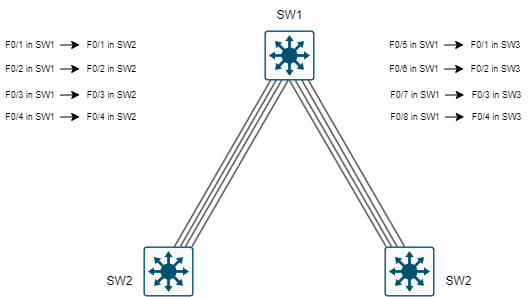
\includegraphics[width=0.9\textwidth]{img/Aggrigation-manual-01.png}
	\caption{\textit{}}
\end{figure}
\newpage
\section{EtherChannel Protocols}
\subsection{Configuring PAgP-based EtherChannel}
\begin{enumerate}
	\item Configure an \textbf{EtherChannel using PAgP} between SW1 and SW2 using interfaces F0/1 - F0/4.

	      %---,,,,,,,,,,,,,,,,,,,,,,,,,,,,,,,,,,---
	      \switchocg{codeblock}{%
		      \color{black}\underline{Click here to display the answer:}%
	      }


	      \begin{ocg}{Code Block}{codeblock}{0}
		      \vspace{0.5cm}
		      Configuration on SW1:
		      \begin{lstlisting}
interface range FastEthernet0/1 - 4
channel-group 1 mode desirable
\end{lstlisting}


		      \vspace{0.5cm}
		      Configuration on SW2:
		      \begin{lstlisting}
interface range FastEthernet0/1 - 4
channel-group 1 mode auto

\end{lstlisting}

	      \end{ocg}
	      %---''''''''''''''''''''''''''''''''---


	\item Verify the EtherChannel status using \texttt{show etherchannel summary} and interpret the output.
	      %---,,,,,,,,,,,,,,,,,,,,,,,,,,,,,,,,,,---
	      \switchocg{codeblock}{%
		      \color{black}\underline{Click here to display the answer:}%
	      }

	      \begin{ocg}{Code Block}{codeblock}{0}

		      \vspace{0.5cm}
		      Verification:
		      \begin{lstlisting}
show etherchannel summary
          \end{lstlisting}

		      \vspace{0.5cm}
		      Expected output:
		      \begin{lstlisting}[columns=fullflexible]
Group  Port-channel  Protocol  Ports  
------ ------------  --------- -------------------
1      Po1          PAgP       Fa0/1(P) Fa0/2(P) Fa0/3(P) Fa0/4(P)
          \end{lstlisting}

	      \end{ocg}
	      %---''''''''''''''''''''''''''''''''---


	\item What happens if one of the links in the EtherChannel fails? Test and analyze.

	      %---,,,,,,,,,,,,,,,,,,,,,,,,,,,,,,,,,,---
	      \switchocg{codeblock}{%
		      \color{black}\underline{Click here to display the answer:}%
	      }

	      \begin{ocg}{Code Block}{codeblock}{0}

		      \vspace{0.5cm}
		      \tcbset{colback=gray!10, colframe=gray!50, boxrule=0.5pt, arc=4pt, left=4pt, right=4pt, top=4pt, bottom=4pt}
		      \begin{tcolorbox}
			      The EtherChannel remains UP with reduced bandwidth
		      \end{tcolorbox}
	      \end{ocg}
	      %---''''''''''''''''''''''''''''''''---


\end{enumerate}

\subsection{Configuring LACP-based EtherChannel}
\begin{enumerate}
	\item Configure an \textbf{EtherChannel using LACP} between SW1 and SW3 using interfaces F0/5 - F0/8.

	      %---,,,,,,,,,,,,,,,,,,,,,,,,,,,,,,,,,,---
	      \switchocg{codeblock}{%
		      \color{black}\underline{Click here to display the answer:}%
	      }

	      \begin{ocg}{Code Block}{codeblock}{0}

		      \vspace{0.5cm}
		      Configuration on SW1:
		      \begin{lstlisting}
interface range FastEthernet0/5 - 8
channel-group 2 mode active
\end{lstlisting}

		      \vspace{0.5cm}
		      Configuration on SW3:
		      \begin{lstlisting}[columns=fullflexible]
interface range FastEthernet0/1 - 4
channel-group 2 mode passive

\end{lstlisting}

	      \end{ocg}
	      %---''''''''''''''''''''''''''''''''---


	\item Change the configuration to use \textbf{LACP Active mode} and check if the channel is formed.

	      %---,,,,,,,,,,,,,,,,,,,,,,,,,,,,,,,,,,---
	      \switchocg{codeblock}{%
		      \color{black}\underline{Click here to display the answer:}%
	      }

	      \begin{ocg}{Code Block}{codeblock}{0}

		      \vspace{0.5cm}
		      Verification:
		      \begin{lstlisting}
show etherchannel summary
\end{lstlisting}

		      \begin{tcolorbox}
			      The status should show Po2 in SU state.
		      \end{tcolorbox}
		      \vspace{0.5cm}
	      \end{ocg}
	      %---''''''''''''''''''''''''''''''''---

	\item What is the difference between \textbf{LACP Active} and \textbf{LACP Passive}?

	      %---,,,,,,,,,,,,,,,,,,,,,,,,,,,,,,,,,,---
	      \switchocg{codeblock}{%
		      \color{black}\underline{Click here to display the answer:}%
	      }

	      \begin{ocg}{Code Block}{codeblock}{0}

		      \vspace{0.5cm}

		      \begin{tcolorbox}
			      \begin{itemize}
				      \item \textbf{Active:} Initiates EtherChannel negotiation.
				      \item \textbf{Passive:} Waits for negotiation requests.
			      \end{itemize}
		      \end{tcolorbox}
		      \vspace{0.5cm}
	      \end{ocg}
	      %---''''''''''''''''''''''''''''''''---

\end{enumerate}

\subsection{Configuring Static Mode EtherChannel}
\begin{enumerate}
	\item Configure an \textbf{EtherChannel in Static Mode (On Mode)} between SW2 and SW3.


	      %---,,,,,,,,,,,,,,,,,,,,,,,,,,,,,,,,,,---
	      \switchocg{codeblock}{%
		      \color{black}\underline{Click here to display the answer:}%
	      }

	      \begin{ocg}{Code Block}{codeblock}{0}

		      \vspace{0.5cm}
		      Configuration on SW2 \& SW3:
		      \begin{lstlisting}
interface range FastEthernet0/1 - 4
channel-group 3 mode on
\end{lstlisting}

		      \vspace{0.5cm}
	      \end{ocg}
	      %---''''''''''''''''''''''''''''''''---




	\item What is the primary risk of using Static Mode instead of PAgP or LACP?


	      %---,,,,,,,,,,,,,,,,,,,,,,,,,,,,,,,,,,---
	      \switchocg{codeblock}{%
		      \color{black}\underline{Click here to display the answer:}%
	      }

	      \begin{ocg}{Code Block}{codeblock}{0}

		      \vspace{0.5cm}
		      \begin{tcolorbox}
			      \textbf{Risk of Static Mode:} No negotiation; mismatched settings cause failure.
		      \end{tcolorbox}
		      \vspace{0.5cm}
	      \end{ocg}
	      %---''''''''''''''''''''''''''''''''---


\end{enumerate}

\subsection{Comparing PAgP, LACP, and Static Mode}
\begin{enumerate}
	\item Comparison table highlighting the \textbf{differences between PAgP, LACP, and Static Mode}.

	      \begin{tabular}{|l|l|l|l|}
		      \hline
		      Feature          & PAgP              & LACP           & Static Mode \\
		      \hline
		      Vendor           & Cisco proprietary & IEEE 802.3ad   & None        \\
		      Negotiation      & Active/Desirable  & Active/Passive & Disabled    \\
		      Redundancy       & High              & High           & Medium      \\
		      Security         & Medium            & High           & Low         \\
		      Failure Handling & Yes               & Yes            & No          \\
		      \hline
	      \end{tabular}

	\item Based on the network topology, which EtherChannel mode would you recommend for maximum reliability?

	      %---,,,,,,,,,,,,,,,,,,,,,,,,,,,,,,,,,,---
	      \switchocg{codeblock}{%
		      \color{black}\underline{Click here to display the answer:}%
	      }

	      \begin{ocg}{Code Block}{codeblock}{0}

		      \vspace{0.5cm}
		      \begin{tcolorbox}
			      Best protocol for this topology? LACP, since it’s vendor-neutral and dynamically negotiates links.
		      \end{tcolorbox}
		      \vspace{0.5cm}
	      \end{ocg}
	      %---''''''''''''''''''''''''''''''''---
\end{enumerate}

\section{Configuring EtherChannel}
\subsection{Full EtherChannel Configuration}
\begin{enumerate}
	\item Configure \textbf{EtherChannel using LACP on SW1 \& SW2} (Interfaces F0/1 - F0/4).
	\item Configure \textbf{EtherChannel using PAgP on SW1 \& SW3} (Interfaces F0/5 - F0/8).

	      %---,,,,,,,,,,,,,,,,,,,,,,,,,,,,,,,,,,---
	      \switchocg{codeblock}{%
		      \color{black}\underline{Click here to display the answer:}%
	      }

	      \begin{ocg}{Code Block}{codeblock}{0}

		      \vspace{0.5cm}
		      Configuration on SW1:
		      \begin{lstlisting}
interface range FastEthernet0/1 - 4
channel-group 1 mode desirable
interface range FastEthernet0/5 - 8
channel-group 2 mode active
    \end{lstlisting}
		      Configuration on SW2:
		      \begin{lstlisting}
interface range FastEthernet0/1 - 4
channel-group 1 mode auto
    \end{lstlisting}
		      Configuration on SW3:
		      \begin{lstlisting}
interface range FastEthernet0/1 - 4
channel-group 2 mode passive
    \end{lstlisting}
		      \vspace{0.5cm}
	      \end{ocg}
	      %---''''''''''''''''''''''''''''''''---

	\item Verify that all EtherChannels are up using \texttt{show etherchannel summary}.
	      %---,,,,,,,,,,,,,,,,,,,,,,,,,,,,,,,,,,---
	      \switchocg{codeblock}{%
		      \color{black}\underline{Click here to display the answer:}%
	      }

	      \begin{ocg}{Code Block}{codeblock}{0}

		      \vspace{0.5cm}
		      \begin{tcolorbox}
			      \texttt{show etherchannel summary} confirms both groups are UP.
		      \end{tcolorbox}
		      \vspace{0.5cm}
	      \end{ocg}
	      %---''''''''''''''''''''''''''''''''---
	\item What does the status flag "SU" indicate in the \texttt{show etherchannel summary} output?

	      %---,,,,,,,,,,,,,,,,,,,,,,,,,,,,,,,,,,---
	      \switchocg{codeblock}{%
		      \color{black}\underline{Click here to display the answer:}%
	      }

	      \begin{ocg}{Code Block}{codeblock}{0}

		      \vspace{0.5cm}

		      \begin{tcolorbox}
			      \begin{itemize}
				      \item \textbf{S} (Layer 2 EtherChannel)
				      \item \textbf{U} (In Use)
			      \end{itemize}
		      \end{tcolorbox}
		      \vspace{0.5cm}
	      \end{ocg}
	      %---''''''''''''''''''''''''''''''''---
\end{enumerate}

\section{Load Balancing in EtherChannel}
\subsection{EtherChannel Load Balancing Methods}
\begin{enumerate}
	\item Configure SW1 to use \textbf{Layer 2 Load Balancing} for EtherChannel.

	      %---,,,,,,,,,,,,,,,,,,,,,,,,,,,,,,,,,,---
	      \switchocg{codeblock}{%
		      \color{black}\underline{Click here to display the answer:}%
	      }

	      \begin{ocg}{Code Block}{codeblock}{0}

		      \vspace{0.5cm}
		      Configuring Layer 2 Load Balancing on SW1
		      \begin{lstlisting}
port-channel load-balance src-mac
    \end{lstlisting}

		      \vspace{0.5cm}
	      \end{ocg}
	      %---''''''''''''''''''''''''''''''''---


	\item Change the configuration to \textbf{Layer 3 Load Balancing} and test using pings.

	      %---,,,,,,,,,,,,,,,,,,,,,,,,,,,,,,,,,,---
	      \switchocg{codeblock}{%
		      \color{black}\underline{Click here to display the answer:}%
	      }

	      \begin{ocg}{Code Block}{codeblock}{0}

		      \vspace{0.5cm}
		      Changing to Layer 3 Load Balancing
		      \begin{lstlisting}
port-channel load-balance src-ip
    \end{lstlisting}

		      \vspace{0.5cm}
	      \end{ocg}
	      %---''''''''''''''''''''''''''''''''---


	\item Use \texttt{show etherchannel load-balance} to verify load balancing mode.
	\item Which load balancing method is best for environments with \textbf{heavy Layer 3 traffic}?
	      Layer 3 method is best for IP-based routing environments.

	      %---,,,,,,,,,,,,,,,,,,,,,,,,,,,,,,,,,,---
	      \switchocg{codeblock}{%
		      \color{black}\underline{Click here to display the answer:}%
	      }

	      \begin{ocg}{Code Block}{codeblock}{0}

		      \vspace{0.5cm}

		      \begin{tcolorbox}
			      Layer 3 method is best for IP-based routing environments.
		      \end{tcolorbox}
		      \vspace{0.5cm}
	      \end{ocg}
	      %---''''''''''''''''''''''''''''''''---


\end{enumerate}

\section{EtherChannel and VLANs}
\subsection{Configuring VLANs with EtherChannel}
\begin{enumerate}
	\item Configure \textbf{VLAN 10 and VLAN 20} on SW1, SW2, and SW3.

	      %---,,,,,,,,,,,,,,,,,,,,,,,,,,,,,,,,,,---
	      \switchocg{codeblock}{%
		      \color{black}\underline{Click here to display the answer:}%
	      }

	      \begin{ocg}{Code Block}{codeblock}{0}

		      \vspace{0.5cm}
		      Configuring VLANs on SW1, SW2, SW3
		      \begin{lstlisting}
vlan 10
vlan 20
\end{lstlisting}

		      \vspace{0.5cm}
	      \end{ocg}
	      %---''''''''''''''''''''''''''''''''---
	\item Assign VLAN 10 to \textbf{EtherChannel between SW1 and SW2}.
	\item Assign VLAN 20 to \textbf{EtherChannel between SW1 and SW3}.

	      %---,,,,,,,,,,,,,,,,,,,,,,,,,,,,,,,,,,---
	      \switchocg{codeblock}{%
		      \color{black}\underline{Click here to display the answer:}%
	      }

	      \begin{ocg}{Code Block}{codeblock}{0}

		      \vspace{0.5cm}
		      Assign VLANs to EtherChannel
		      \begin{lstlisting}
interface port-channel 1
switchport mode access
switchport access vlan 10
\end{lstlisting}

		      \vspace{0.5cm}
	      \end{ocg}
	      %---''''''''''''''''''''''''''''''''---

	\item Verify VLAN configuration with \texttt{show vlan brief}.
\end{enumerate}

\subsection{EtherChannel with Trunking}
\begin{enumerate}
	\item Configure the EtherChannel between SW1 and SW2 as a \textbf{trunk port}.

	      %---,,,,,,,,,,,,,,,,,,,,,,,,,,,,,,,,,,---
	      \switchocg{codeblock}{%
		      \color{black}\underline{Click here to display the answer:}%
	      }

	      \begin{ocg}{Code Block}{codeblock}{0}

		      \vspace{0.5cm}
		      Configure trunking on EtherChannel between SW1 \& SW2
		      \begin{lstlisting}
interface port-channel 1
switchport mode trunk
\end{lstlisting}

		      \vspace{0.5cm}
	      \end{ocg}
	      %---''''''''''''''''''''''''''''''''---





	\item Allow \textbf{only VLANs 10 and 20} on the trunk.

	      %---,,,,,,,,,,,,,,,,,,,,,,,,,,,,,,,,,,---
	      \switchocg{codeblock}{%
		      \color{black}\underline{Click here to display the answer:}%
	      }

	      \begin{ocg}{Code Block}{codeblock}{0}

		      \vspace{0.5cm}
		      Allow VLANs 10 and 20 on the trunk On SW1 and SW2:
		      \begin{lstlisting}
interface port-channel 1
switchport trunk allowed vlan 10,20
    \end{lstlisting}

		      \vspace{0.5cm}
	      \end{ocg}
	      %---''''''''''''''''''''''''''''''''---



	\item Verify trunking using \texttt{show interfaces trunk}.
\end{enumerate}

\subsection{VLAN Load Distribution}
\begin{enumerate}
	\item Configure VLAN load balancing on EtherChannel using \textbf{MAC address-based hashing}.

	      %---,,,,,,,,,,,,,,,,,,,,,,,,,,,,,,,,,,---
	      \switchocg{codeblock}{%
		      \color{black}\underline{Click here to display the answer:}%
	      }

	      \begin{ocg}{Code Block}{codeblock}{0}

		      \vspace{0.5cm}
		      Configure MAC-based VLAN load balancing On SW1
		      \begin{lstlisting}
port-channel load-balance src-mac
\end{lstlisting}

		      \vspace{0.5cm}
	      \end{ocg}
	      %---''''''''''''''''''''''''''''''''---


	\item Change the hashing method to \textbf{IP-based} and test using pings from multiple VLANs.

	      %---,,,,,,,,,,,,,,,,,,,,,,,,,,,,,,,,,,---
	      \switchocg{codeblock}{%
		      \color{black}\underline{Click here to display the answer:}%
	      }

	      \begin{ocg}{Code Block}{codeblock}{0}

		      \vspace{0.5cm}
		      Change to IP-based load balancing On SW1
		      \begin{lstlisting}
port-channel load-balance src-ip
\end{lstlisting}

		      Verify Load Balancing:

		      \begin{lstlisting}
show etherchannel load-balance
\end{lstlisting}


		      \vspace{0.5cm}
	      \end{ocg}
	      %---''''''''''''''''''''''''''''''''---

\end{enumerate}

\subsection{Troubleshooting VLAN and EtherChannel Issues}
\begin{enumerate}
	\item Intentionally misconfigure VLANs in EtherChannel and analyze error messages.

	      %---,,,,,,,,,,,,,,,,,,,,,,,,,,,,,,,,,,---
	      \switchocg{codeblock}{%
		      \color{black}\underline{Click here to display the answer:}%
	      }

	      \begin{ocg}{Code Block}{codeblock}{0}

		      \vspace{0.5cm}
		      Misconfigure VLANs intentionally On SW1:
		      \begin{lstlisting}
interface port-channel 1
switchport access vlan 30
\end{lstlisting}

		      Expected Error Message

		      \begin{lstlisting}
% Access VLAN does not match on both sides of the EtherChannel
\end{lstlisting}

		      \begin{tcolorbox}
			      Fix: Ensure VLAN settings match on both ends.
		      \end{tcolorbox}


		      \vspace{0.5cm}
	      \end{ocg}
	      %---''''''''''''''''''''''''''''''''---
	\item Use \texttt{show spanning-tree} to check if there are blocked ports.


	\item What happens if VLANs are not allowed on both EtherChannel sides?


	      %---,,,,,,,,,,,,,,,,,,,,,,,,,,,,,,,,,,---
	      \switchocg{codeblock}{%
		      \color{black}\underline{Click here to display the answer:}%
	      }

	      \begin{ocg}{Code Block}{codeblock}{0}

		      \vspace{0.5cm}


		      \begin{tcolorbox}
			      If VLANs are not allowed on both sides, devices in that VLAN won’t communicate.\\
			      Fix: Ensure VLAN consistency.
		      \end{tcolorbox}


		      \vspace{0.5cm}
	      \end{ocg}
	      %---''''''''''''''''''''''''''''''''---

\end{enumerate}


\section{Advanced EtherChannel Troubleshooting}
\subsection{Identifying Common Problems}
\begin{enumerate}
	\item Configure EtherChannel with \textbf{one mismatched mode} (PAgP on one switch and LACP on the other).


	      %---,,,,,,,,,,,,,,,,,,,,,,,,,,,,,,,,,,---
	      \switchocg{codeblock}{%
		      \color{black}\underline{Click here to display the answer:}%
	      }

	      \begin{ocg}{Code Block}{codeblock}{0}

		      \vspace{0.5cm}

		      Mismatched Protocols (PAgP on SW1, LACP on SW2)

		      On SW1:
		      \begin{lstlisting}
interface range FastEthernet0/1 - 4
channel-group 1 mode desirable
\end{lstlisting}

		      On SW2:
		      \begin{lstlisting}
interface range FastEthernet0/1 - 4
channel-group 1 mode active
\end{lstlisting}
		      \vspace{0.5cm}
	      \end{ocg}
	      %---''''''''''''''''''''''''''''''''---
	\item Analyze the \textbf{error messages} and explain why EtherChannel fails.

	      %---,,,,,,,,,,,,,,,,,,,,,,,,,,,,,,,,,,---
	      \switchocg{codeblock}{%
		      \color{black}\underline{Click here to display the answer:}%
	      }

	      \begin{ocg}{Code Block}{codeblock}{0}

		      \vspace{0.5cm}

		      Expected Error Message:
		      \begin{lstlisting}
% EC-5-LIMITEXCEEDED: Too many unbundled ports in channel
\end{lstlisting}
		      \begin{tcolorbox}
			      Fix: Ensure both switches use the same protocol.
		      \end{tcolorbox}


		      \vspace{0.5cm}
	      \end{ocg}
	      %---''''''''''''''''''''''''''''''''---
	\item How does EtherChannel react when one switch is powered off?


	      %---,,,,,,,,,,,,,,,,,,,,,,,,,,,,,,,,,,---
	      \switchocg{codeblock}{%
		      \color{black}\underline{Click here to display the answer:}%
	      }

	      \begin{ocg}{Code Block}{codeblock}{0}

		      \vspace{0.5cm}

		      \begin{tcolorbox}
			      \begin{itemize}
				      \item EtherChannel between SW1 and SW2 fails over to remaining active links.
				      \item If STP is not correctly configured, loops may occur.
			      \end{itemize}

		      \end{tcolorbox}


		      \vspace{0.5cm}
	      \end{ocg}
	      %---''''''''''''''''''''''''''''''''---
\end{enumerate}

\subsection{Using Show Commands}
\begin{enumerate}
	\item Use \texttt{show etherchannel summary} and analyze the output.

	      %---,,,,,,,,,,,,,,,,,,,,,,,,,,,,,,,,,,---
	      \switchocg{codeblock}{%
		      \color{black}\underline{Click here to display the answer:}%
	      }

	      \begin{ocg}{Code Block}{codeblock}{0}

		      \vspace{0.5cm}

		      Check EtherChannel Summary:
		      \begin{lstlisting}
show etherchannel summary
    \end{lstlisting}

		      Output Analysis:
		      \begin{tcolorbox}
			      \begin{itemize}
				      \item \texttt{SU} → EtherChannel is up.
				      \item \texttt{D} → EtherChannel is down.
			      \end{itemize}
		      \end{tcolorbox}


		      \vspace{0.5cm}
	      \end{ocg}
	      %---''''''''''''''''''''''''''''''''---
	\item Use \texttt{show spanning-tree} to verify how STP interacts with EtherChannel.

	      %---,,,,,,,,,,,,,,,,,,,,,,,,,,,,,,,,,,---
	      \switchocg{codeblock}{%
		      \color{black}\underline{Click here to display the answer:}%
	      }

	      \begin{ocg}{Code Block}{codeblock}{0}

		      \vspace{0.5cm}

		      Check STP:
		      \begin{lstlisting}
show spanning-tree
        \end{lstlisting}


		      \begin{tcolorbox}
			      Look for blocked ports due to STP loops.
		      \end{tcolorbox}


		      \vspace{0.5cm}
	      \end{ocg}
	      %---''''''''''''''''''''''''''''''''---


	\item Use \texttt{debug etherchannel} to track EtherChannel negotiation.

	      %---,,,,,,,,,,,,,,,,,,,,,,,,,,,,,,,,,,---
	      \switchocg{codeblock}{%
		      \color{black}\underline{Click here to display the answer:}%
	      }

	      \begin{ocg}{Code Block}{codeblock}{0}

		      \vspace{0.5cm}

		      Debugging EtherChannel:
		      \begin{lstlisting}
debug etherchannel
        \end{lstlisting}


		      \begin{tcolorbox}
			      Track EtherChannel negotiation logs.
		      \end{tcolorbox}


		      \vspace{0.5cm}
	      \end{ocg}
	      %---''''''''''''''''''''''''''''''''---


\end{enumerate}

\subsection{Best Practices in Troubleshooting}
\begin{enumerate}
	\item What are the three most common reasons for EtherChannel failure?

	      %---,,,,,,,,,,,,,,,,,,,,,,,,,,,,,,,,,,---
	      \switchocg{codeblock}{%
		      \color{black}\underline{Click here to display the answer:}%
	      }

	      \begin{ocg}{Code Block}{codeblock}{0}

		      \vspace{0.5cm}

		      \begin{tcolorbox}
			      \begin{itemize}
				      \item Mismatched protocols (PAgP vs LACP vs Static).
				      \item Speed/Duplex mismatches on bundled ports.
				      \item Trunk/access mode conflicts.
			      \end{itemize}
		      \end{tcolorbox}

		      \begin{tcolorbox}
			      Check all these before troubleshooting further!
		      \end{tcolorbox}



		      \vspace{0.5cm}
	      \end{ocg}
	      %---''''''''''''''''''''''''''''''''---


	\item How can \textbf{Port Speed/Duplex mismatches} affect EtherChannel?


	      %---,,,,,,,,,,,,,,,,,,,,,,,,,,,,,,,,,,---
	      \switchocg{codeblock}{%
		      \color{black}\underline{Click here to display the answer:}%
	      }

	      \begin{ocg}{Code Block}{codeblock}{0}

		      \vspace{0.5cm}
		      EtherChannel requires all member interfaces to have the same:


		      \begin{tcolorbox}
			      \begin{itemize}
				      \item Speed (e.g., 1000 Mbps)
				      \item Duplex mode (Full or Half)
			      \end{itemize}
		      \end{tcolorbox}


		      Example Mismatch Check:
		      \begin{lstlisting}
show interfaces FastEthernet0/1 status
                \end{lstlisting}
		      Solution:
		      \begin{lstlisting}
interface range FastEthernet0/1 - 4
speed 1000
duplex full
            \end{lstlisting}



		      \vspace{0.5cm}
	      \end{ocg}
	      %---''''''''''''''''''''''''''''''''---

	\item What steps should you take if an EtherChannel is \textbf{partially up}?
	

     %---,,,,,,,,,,,,,,,,,,,,,,,,,,,,,,,,,,---
     \switchocg{codeblock}{%
     \color{black}\underline{Click here to display the answer:}%
 }

 \begin{ocg}{Code Block}{codeblock}{0}

     \vspace{0.5cm}
     Step 1: Verify Active Links
     \begin{lstlisting}
show etherchannel summary
    \end{lstlisting}
    \begin{itemize}
        \item \small If some ports are in (D) Down state, check for errors.
    \end{itemize}
    

    Step 2: Check Port Status
    \begin{lstlisting}
show interfaces status
    \end{lstlisting}
    \begin{itemize}
        \item \small Look for err-disabled or shutdown ports.
    \end{itemize}


    Step 3: Reset the EtherChannel
    \begin{lstlisting}
interface port-channel 1
shutdown
no shutdown
    \end{lstlisting}
    \begin{itemize}
        \item \small Sometimes, reinitializing the interface resolves issues.
    \end{itemize}

     \vspace{0.5cm}
 \end{ocg}
 %---''''''''''''''''''''''''''''''''---

\end{enumerate}

\subsection{Real-World Case Study}
\begin{enumerate}
	\item Read the following network issue scenario and propose a solution:
	      \begin{itemize}
		      \item "EtherChannel between SW1 and SW2 goes down when adding a new link. Removing the link restores the channel."
		      \item What is the most likely cause?

		            %---,,,,,,,,,,,,,,,,,,,,,,,,,,,,,,,,,,---
		            \switchocg{codeblock}{%
			            \color{black}\underline{Click here to display the answer:}%
		            }

		            \begin{ocg}{Code Block}{codeblock}{0}

			            \vspace{0.5cm}

			            \begin{tcolorbox}
				            \begin{itemize}
					            \item New interface has mismatched speed, duplex, or VLAN settings.
					            \item EtherChannel bundle only allows similar interfaces.
				            \end{itemize}
			            \end{tcolorbox}



			            \vspace{0.5cm}
		            \end{ocg}
		            %---''''''''''''''''''''''''''''''''---
		      \item How can you prevent this from happening?


		            %---,,,,,,,,,,,,,,,,,,,,,,,,,,,,,,,,,,---
		            \switchocg{codeblock}{%
			            \color{black}\underline{Click here to display the answer:}%
		            }

		            \begin{ocg}{Code Block}{codeblock}{0}

			            \vspace{0.5cm}
			            Check the new link’s settings:
			            \begin{lstlisting}
show interfaces FastEthernet0/x
                                    \end{lstlisting}


			            \begin{tcolorbox}
				            Ensure it matches existing EtherChannel settings.
			            \end{tcolorbox}



			            \vspace{0.5cm}
		            \end{ocg}
		            %---''''''''''''''''''''''''''''''''---
	      \end{itemize}
\end{enumerate}


\section{Best Practices and Security Considerations}
\subsection{EtherChannel Best Practices}
\begin{enumerate}
	\item List five best practices for deploying EtherChannel in a production network.

	      %---,,,,,,,,,,,,,,,,,,,,,,,,,,,,,,,,,,---
	      \switchocg{codeblock}{%
		      \color{black}\underline{Click here to display the answer:}%
	      }

	      \begin{ocg}{Code Block}{codeblock}{0}

		      \vspace{0.5cm}

		      \textbf{Key Best Practices:}
		      \begin{tcolorbox}
			      \begin{itemize}
				      \item Use LACP Instead of PAgP or Static Mode
				      \item Ensure Matching Configurations on Both Ends
				      \item Implement Load Balancing Based on Traffic Type
				      \item Monitor EtherChannel Status and Performance
				      \item Enable STP Protection Features (BPDU Guard \& Root Guard)
			      \end{itemize}
		      \end{tcolorbox}

		      \vspace{0.5cm}
	      \end{ocg}
	      %---''''''''''''''''''''''''''''''''---


	\item What are the risks of \textbf{misconfigured EtherChannel}?


	      %---,,,,,,,,,,,,,,,,,,,,,,,,,,,,,,,,,,---
	      \switchocg{codeblock}{%
		      \color{black}\underline{Click here to display the answer:}%
	      }

	      \begin{ocg}{Code Block}{codeblock}{0}

		      \medskip

		      \centering
		      \begin{tcolorbox}
			      \centering
			      \resizebox{\textwidth}{!}{ % Automatically resizes the table to fit
				      \begin{tabular}{|l|l|}
					      \hline
					      \textbf{Misconfiguration}                                      & \textbf{Potential Impact}               \\
					      \hline
					      Mismatched LACP/PAgP settings                                  & EtherChannel fails to establish         \\
					      Inconsistent VLAN configuration                                & VLAN traffic loss                       \\
					      Speed/Duplex mismatch                                          & Poor performance, packet drops          \\
					      One side configured as EtherChannel, other as individual links & Packet duplication, network instability \\
					      Spanning Tree not adjusted for EtherChannel                    & STP blocking active links               \\
					      \hline
				      \end{tabular}
			      }
		      \end{tcolorbox}


		      \medskip
	      \end{ocg}
	      %---''''''''''''''''''''''''''''''''---

\end{enumerate}

\subsection{Security Risks}
\begin{enumerate}
	\item How can EtherChannel be exploited in a \textbf{MAC spoofing attack}?

	      %---,,,,,,,,,,,,,,,,,,,,,,,,,,,,,,,,,,---
	      \switchocg{codeblock}{%
		      \color{black}\underline{Click here to display the answer:}%
	      }

	      \begin{ocg}{Code Block}{codeblock}{0}

		      \vspace{0.5cm}

		      \begin{tcolorbox}
			      \begin{itemize}
				      \item Attackers can spoof MAC addresses to trick the switch into sending traffic over a specific EtherChannel link.
				      \item This allows traffic interception, man-in-the-middle (MITM) attacks, or session hijacking.
				      \item If EtherChannel is misconfigured, it may forward traffic unpredictably, leading to data leaks.
			      \end{itemize}
		      \end{tcolorbox}

		      \vspace{0.5cm}
	      \end{ocg}
	      %---''''''''''''''''''''''''''''''''---
	\item What security measures can prevent \textbf{EtherChannel-based attacks}?


	      %---,,,,,,,,,,,,,,,,,,,,,,,,,,,,,,,,,,---
	      \switchocg{codeblock}{%
		      \color{black}\underline{Click here to display the answer:}%
	      }

	      \begin{ocg}{Code Block}{codeblock}{0}

		      \vspace{0.5cm}

		      Implement Port Security on EtherChannel:

		      \begin{lstlisting}
interface port-channel 1
switchport port-security
switchport port-security maximum 3
switchport port-security violation restrict
            \end{lstlisting}
		      \begin{itemize}
			      \item \small Limits the number of MAC addresses on the EtherChannel.
		      \end{itemize}
		      \vspace{1cm}

		      Enable BPDU Guard to Prevent Rogue Switches:
		      \begin{lstlisting}
spanning-tree bpduguard enable
            \end{lstlisting}

		      \begin{itemize}
			      \item \small Prevents unauthorized STP BPDU injections, stopping attackers from modifying the spanning-tree topology.
		      \end{itemize}
		      \vspace{1cm}

		      Use Dynamic ARP Inspection (DAI):
		      \begin{lstlisting}
ip arp inspection vlan 10,20
            \end{lstlisting}

		      \begin{itemize}
			      \item \small Stops MAC spoofing by validating ARP packets.
		      \end{itemize}
		      \vspace{1cm}


		      Enable DHCP Snooping to Prevent Rogue DHCP Servers:
		      \begin{lstlisting}
ip dhcp snooping
ip dhcp snooping vlan 10,20
            \end{lstlisting}

		      \begin{itemize}
			      \item \small Prevents rogue devices from issuing IP addresses.
		      \end{itemize}

		      \vspace{0.5cm}
	      \end{ocg}
	      %---''''''''''''''''''''''''''''''''---
\end{enumerate}

\subsection{Securing EtherChannel Configurations}
\begin{enumerate}
	\item Configure \textbf{BPDU Guard} and \textbf{Root Guard} on EtherChannel links.

	      %---,,,,,,,,,,,,,,,,,,,,,,,,,,,,,,,,,,---
	      \switchocg{codeblock}{%
		      \color{black}\underline{Click here to display the answer:}%
	      }

	      \begin{ocg}{Code Block}{codeblock}{0}

		      \vspace{0.5cm}

		      Enable BPDU Guard on Access Layer Switches (Prevents Rogue STP BPDUs):
		      \begin{lstlisting}
interface port-channel 1
spanning-tree bpduguard enable
    \end{lstlisting}
		      \begin{itemize}
			      \item \small Effect: If an unauthorized switch sends BPDU packets, the interface is shut down.
		      \end{itemize}
		      \vspace{1cm}
		      Enable Root Guard on Distribution/Core Switches:
		      \begin{lstlisting}
interface port-channel 1
spanning-tree guard root
            \end{lstlisting}

		      \begin{itemize}
			      \item \small Effect: Prevents rogue switches from taking over the STP root role.
		      \end{itemize}
		      \vspace{0.5cm}
	      \end{ocg}
	      %---''''''''''''''''''''''''''''''''---
	\item Why is \textbf{STP Loop Protection} important in an EtherChannel environment?

	      %---,,,,,,,,,,,,,,,,,,,,,,,,,,,,,,,,,,---
	      \switchocg{codeblock}{%
		      \color{black}\underline{Click here to display the answer:}%
	      }

	      \begin{ocg}{Code Block}{codeblock}{0}

		      \vspace{0.5cm}
		      \begin{tcolorbox}
			      \begin{itemize}
				      \item If an EtherChannel misconfiguration causes links to act independently, STP may not recognize them as a single logical link.
				      \item This can lead to forwarding loops, causing network-wide outages.
				      \item Using BPDU Guard and Root Guard helps prevent STP topology changes.
			      \end{itemize}
		      \end{tcolorbox}

		      \begin{itemize}
			      \item \small Best Practice: Run \texttt{show spanning-tree} to confirm STP status.
		      \end{itemize}
	      \end{ocg}
	      %---''''''''''''''''''''''''''''''''---


\end{enumerate}

\end{document}
